\begin{activity} \label{A:2.7.1}  
Consider the curve defined by the equation $x = y^5 - 5y^3 + 4y$, whose graph is pictured in Figure~\ref{F:2.7.Act1}.
\begin{figure}[h]
\begin{center}
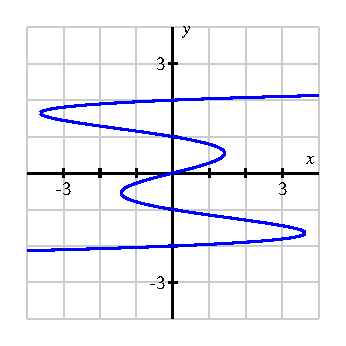
\includegraphics{figures/2_7_Act1.eps}
\caption{The curve $x = y^5 - 5y^3 + 4y$.} \label{F:2.7.Act1}
\end{center}
\end{figure}
\ba
	\item Explain why it is not possible to express $y$ as an explicit function of $x$.

	\item Use implicit differentiation to find a formula for $dy/dx$.

	\item Use your result from part (b) to find an equation of the line tangent to the graph of $x = y^5 -
5y^3 + 4y$ at the point $(0, 1)$.

	\item Use your result from part (b) to determine all of the points at
which the graph of $x = y^5 - 5y^3 + 4y$ has a vertical tangent
line.
\ea
\end{activity}
\begin{smallhint}
\ba
	\item Does the graph pass the vertical line test?
	\item Note, for instance, that $\frac{d}{dx}[y^5] = 5y^4$.
	\item Remember the meaning of $\left. \frac{dy}{dx} \right|_{(0,1)}$.
	\item What is the slope of a vertical line?
\ea
\end{smallhint}
\begin{bighint}
\ba
	\item Does the graph pass the vertical line test?  Can you solve the degree 5 equation $x = y^5 - 5y^3 + 4y$ for $y$?
	\item Note, for instance, that $\frac{d}{dx}[y^5] = 5y^4$.  After differentiating, factor to get a single instance of $\frac{dy}{dx}$ on one side of the equation.
	\item Remember the meaning of $\left. \frac{dy}{dx} \right|_{(0,1)}$ and that point-slope form of a line is $y - y_0 = m(x-x_0)$.
	\item A line is vertical if and only if its slope is undefined.  What point(s) make $\frac{dy}{dx}$ undefined?
\ea
\end{bighint}
\begin{activitySolution}
\ba
	\item Because the graph of the curve fails the vertical line test, $y$ cannot be a function of $x$.  This also confirms our intuition that there is not an algebraic means by which we can rearrange the equation $x = y^5 - 5y^3 + 4y$ to write $y$ in terms of $x$.
	\item We differentiate implicitly, taking the derivative of each side with respect to $x$,
	$$\frac{d}{dx}[x ]= \frac{d}{dx}[y^5 - 5y^3 + 4y],$$
	and evaluate the elementary derivative on the left and use the sum rule on the right to find that
	$$1 = \frac{d}{dx}[y^5] - \frac{d}{dx}[5y^3] + \frac{d}{dx}[4y].$$
	By the chain and constant multiple rules, viewing $y$ as a function of $x$, we now have
	$$1 = 5y^4\frac{dy}{dx} - 15y^2\frac{dy}{dx} + 4\frac{dy}{dx}.$$
	Factoring,
	$$1 = \frac{dy}{dx}(5y^4 - 15y^2 + 4),$$
	and therefore
	$$\frac{dy}{dx} = \frac{1}{5y^4 - 15y^2 + 4}.$$
	\item To find an equation of the line tangent to the graph of $x = y^5 - 5y^3 + 4y$ at the point $(0, 1)$, we only need the slope of the tangent line.  Hence we compute 
	$$\left. \frac{dy}{dx} \right|_{(0,1)} = \frac{1}{5 \cdot 1^4 - 15 \cdot 1^2 + 4} = -\frac{1}{6}.$$
	Therefore, the equation of the tangent line is
	$$y - 1 = -\frac{1}{6}(x-0)$$
	or $y = -\frac{1}{6}x + 1$.
	\item Since a line is vertical whenever its slope is undefined, we seek all points $(x,y)$ that make $\frac{dy}{dx}$ undefined.  This will occur precisely when the denominator, $5y^4 - 15y^2 + 4$, is zero.  Using a graphing utility or computer algebra system to solve the equation $5y^4 - 15y^2 + 4 = 0$, we find that this happens at the four approximate $y$-values $y \approx \pm 0.543912, \pm 1.64443$.  For each such value, we use the original equation $x = y^5 - 5y^3 + 4y$ to find the $x$-value of the point.  Doing so, we have established that there are four points at which the tangent line is vertical, and they are approximately $(1.418697,0.543912)$, $(-1.418697,-0.543912)$, $(-3.63143, 1.64443)$, and $(3.63143, -1.64443)$. 
\ea
\end{activitySolution}
\aftera